\section{O básico de um external}


\begin{frame}[fragile]{O mínimo para um \external (1/2)}
\noindent
1. Um tipo e uma estrutura que representam uma classe: 
\begin{lstlisting}
static t_class *example1_class;

typedef struct _example1 {
  t_object x_obj;
} t_example1;
\end{lstlisting}
2. Uma função de configuração da classe:
\begin{lstlisting}[firstnumber=last]
void example1_setup(void) {
  example1_class = class_new(
    gensym("example1"),         // Nome simbolico
    (t_newmethod) example1_new, // Construtor
    0,                          // Destrutor
    sizeof (t_example1),        // Atributos
    CLASS_NOINLET,              // Flags da classe
    0                           // Tipos
  );
}
\end{lstlisting}
\end{frame}


\begin{frame}[fragile]{O mínimo para um \external (2/2)}
\noindent
3. Um método construtor:
\begin{lstlisting}[firstnumber=last]
// Construtor da classe
void * example1_new(void) {
    t_example1 *x = (t_example1 *) pd_new(example1_class);
    return (void *) x;
}
\end{lstlisting}
\end{frame}


\begin{frame}[fragile]{Bibliotecas (1/2)}
Podemos definir diversas classes numa mesma função de inicialização:
\begin{lstlisting}
void example2_setup(void) {
  post("Initializing my library");

  myobj1_class = class_new(
    gensym("myobj1"),
    (t_newmethod) myobj1_new, // Constructor
    0,
    sizeof (t_myobj1),
    CLASS_NOINLET,
    0);

  myobj2_class = class_new(
    gensym("myobj2"),
    (t_newmethod) myobj2_new, // Constructor
    0,
    sizeof (t_myobj2),
    CLASS_NOINLET,
    0);
}
\end{lstlisting}
\end{frame}


\begin{frame}[fragile]{Bibliotecas (2/2)}
\begin{figure}
\centering
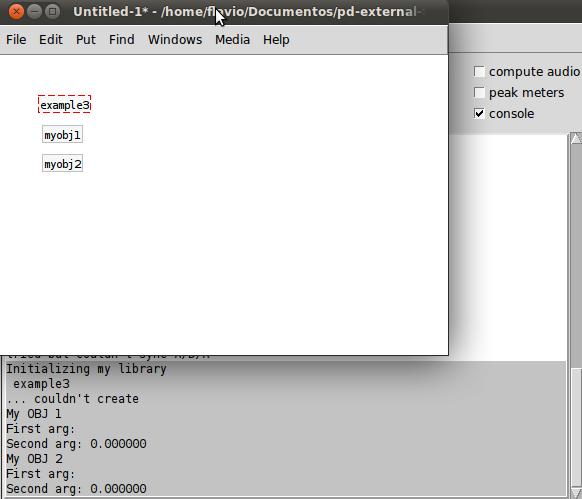
\includegraphics[width=0.7\textwidth]{example3}
\end{figure}
\end{frame}


\begin{frame}[fragile]{Variáveis globais}
Variáveis globais são acessadas por todas as instâncias de objetos e funções
do \external:
\begin{lstlisting}
int count = 0;
void * example4_new(void) {
    t_example4 *x = (t_example4 *) pd_new(example4_class);
    post("Counter value: %d",count);
    count++;
    return (void *) x;
}
\end{lstlisting}
\end{frame}


\begin{frame}[fragile]{Variáveis de instância}
Variáveis declaradas dentro da estrutura de uma classe são como atributos dos
objetos:
\begin{lstlisting}
static t_class *example_class;

typedef struct _example {
    t_object x_obj;
    t_int counter;
} t_example;

void * example_new(void) {
    t_example *x = (t_example *)pd_new(example_class);
    post("Counter value: %d",x->counter);
    x->counter++;
    return (void *) x;
}
\end{lstlisting}
\end{frame}

